\documentclass{beamer}
\mode<presentation>{
\usetheme{Warsaw}
\useoutertheme{infolines}
\useinnertheme{rounded}
\setbeamercovered{transparent}
\setbeamertemplate{theorems}[numbered]
\usecolortheme{rose}
}
\usepackage{multicol}
\usepackage[english]{babel}
\usepackage{amsmath}
\usepackage{amsfonts}
\usepackage{amssymb}
\usepackage{graphicx}
\usepackage{subfigure}
\usepackage{color}
\setbeamertemplate{caption}[numbered]%number the picture


\begin{document}
\title{Graduation Project}
\subtitle{Optimization of the Adaptive Matching Method for Indoor Environment Based on Binocular Vision}
\author{Yu-Fei Zhang}
\date{\today}

\renewcommand{\raggedright}{\leftskip=0pt \rightskip=0pt plus 0cm}


\begin{frame}
\titlepage
\end{frame}


\begin{frame}
\frametitle{Content}
\tableofcontents
\end{frame}

\section{Project background and meaning}
\subsection{Introduction of Stereo Matching}
\begin{frame}
\frametitle{1.1 Introduction of Stereo Matching}


\begin{figure}
\centering
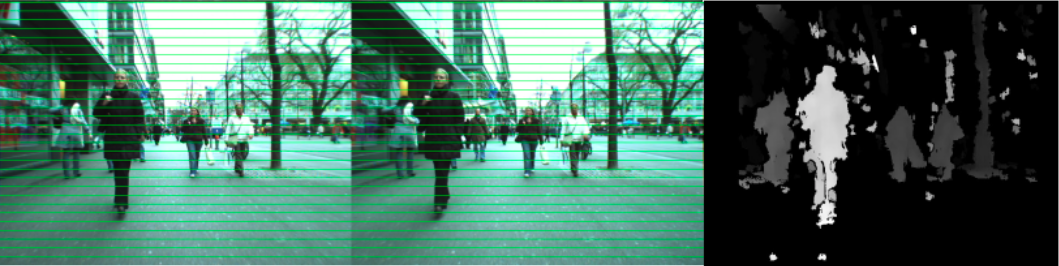
\includegraphics[width=4.5in]{timg-4.png}
\caption{Stereo Matching}
\end{figure}


\raggedright ~~As an important branch of computer vision, stereo matching aims to extract three-dimensional information from two-dimensional images and restore the three-dimensional scene.



\end{frame}

\subsection{Application of Stereo Matching}
\begin{frame}
\frametitle{1.2 Application of Stereo Matching}

\begin{figure}
\centering
\subfigure[Machine inspection]{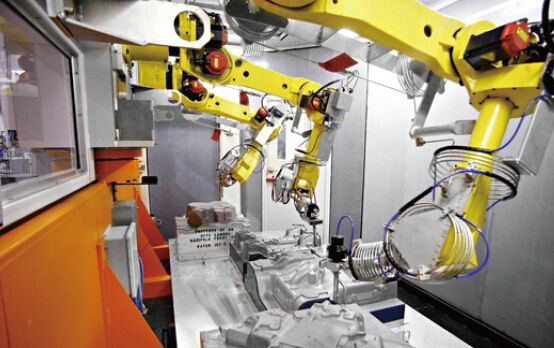
\includegraphics[width=1.4in,height=1.1in]{timg.png}}
\subfigure[Fingerprint recognition]{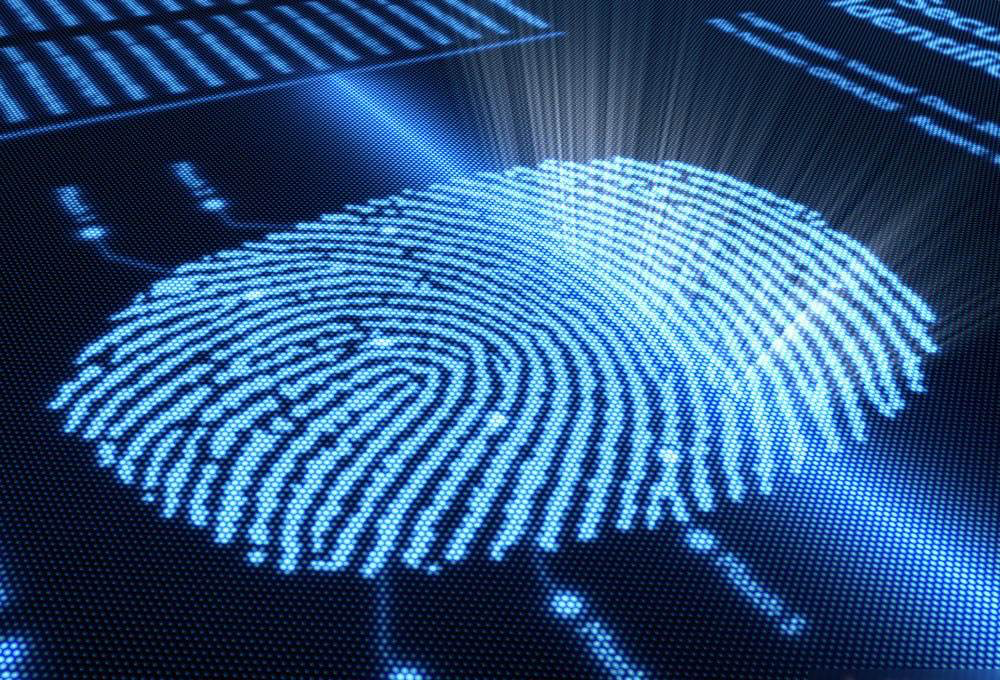
\includegraphics[width=1.4in,height=1.1in]{timg-3.png}}
\subfigure[Face detection]{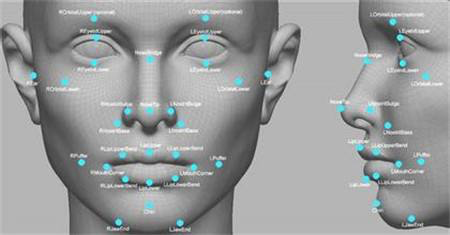
\includegraphics[width=1.4in,height=1.1in]{timg-2.png}}
\caption{Application of stereo matching}
\end{figure}

~~Industrial application : Machine inspection, Fingerprint recognition, Face detection, 3D reconstruction and etc.
\end{frame}

\subsection{Classification of Stereo Matching}
\begin{frame}
\frametitle{1.3 Classification of stereo matching}
~~According to the optimization theory used, stereo matching algorithm can be divided to global matching algorithm and local matching algorithm.

\begin{table}
\centering
\caption{Classification of stereo matching}
\begin{tabular}{|c|c|c|c|}
\hline
Type & Time & Accuracy & Example\\
\hline
Global & long & high & graph cuts, belief propagation\\
\hline
Local & short & low & SAD, SSD, NCC, ASW\\
\hline
\end{tabular}
\end{table}

~~ASW(Adaptive Support-weight) algorithm is one of the most accurate local matching algorithms, while it consumes much time to calculate weights because of its high computational complexity and needs to be improved.


\end{frame}


\section{Research work}
\begin{frame}
\frametitle{2. Research work}
\begin{enumerate}
\item Using the 4 standard image test pair supported by stereo matching standard test platform, study and experimentally analyze current local matching algorithms, including SAD, SSD, NCC and ASW.

\item Optimize the ASW algorithm by simplifying its color support-weight function 

\item Add subsequently processes to the original disparity map, including left-right continuity test, occluded filling and median filtering.
\end{enumerate}
\end{frame}

\section{Fundamental principles}
\subsection{Stereo matching principle}
\begin{frame}
\frametitle{3.1 Stereo matching principle}
\begin{multicols}{2}


\begin{figure}[!htp]
\centering
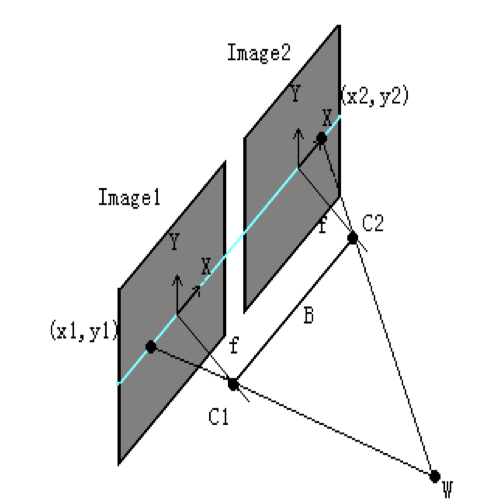
\includegraphics[width=2in]{Picture1.png}
\caption{Binocular imaging}\label{fig 1}
\end{figure}

\columnbreak
\begin{itemize}
\item Disparity : $B$ is the optical center distance of two cameras, $f$ is the focal distance, $(x1,y1)$, $(x2,y2)$ are the position of point $w$ respectively on the left image and the right image. Then $d=|x1-x2|$ is the disparity of two 2D points.

\item Based on the pixel disparity, we can restore its 3D information according to the principle of projection geometry.
\end{itemize}
\end{multicols}
\end{frame}

\subsection{Principle of SAD, SSD and NCC}
\begin{frame}
\frametitle{3.2 Principle of SAD, SSD and NCC}
Suppose that $p_i$ and $p_j$ are the gray values of the matching points and candidate matching points, the matching cost of each algorithm is as follows :
\begin{itemize}
\item SAD(Sum of Absolute Difference) :
\begin{equation}
C_{SAD}=\sum(p_i-p_j)
\end{equation}

\item SSD(Sum of Square Difference) :
\begin{equation}
C_{SSD}=\sum(p_i-p_j)^2
\end{equation}

\item NCC(Normalized Cross Correlation) :
\begin{equation}
C_{NCC}=\frac{\sum p_ip_j}{\sqrt{\sum p_i^2 p_j^2}}
\end{equation}
\end{itemize}
\end{frame}

\subsection{Principle of ASW}
\begin{frame}
\frametitle{3.3 Principle of ASW}
Suppose that $p$ is the pixel to be matched in the left view, $q$ is a pixel in the support window of the left view, the support weight of the pixel point $p$ for pixel point $q$ is :
\begin{equation}
w(p,q)=f(\Delta c_{pq})\cdot f(\Delta g_{pq})
\end{equation}
where $f(\Delta c_{pq})$ represent the color similarity of $p$ and $q$, $f(\Delta g_{pq})$ represent the spatial similarity of $p$ and $q$.

Then the matching cost of $p$ and $\overline{p_d}$ is given as follow :

\begin{equation}
E(p,\overline{p_d}) = \frac {\sum_{q\in N_p,\overline{q}\in N_{\overline{p_d}}}w(p,q)w(\overline{p_d},\overline{q_d})e_0(q,\overline{q_d})} {\sum_{q\in N_p,\overline{q}\in N_{\overline{p_d}}}w(p,q)w(\overline{p_d},\overline{q_d})}
\end{equation}

\end{frame}

\section{Research achievement}
\subsection{Experimental analysis of local matching algorithms}
\begin{frame}
\frametitle{4.1.1 Disparity maps of SAD, SSD, NCC and ASW}
Take Teddy test pair for example, matching window $11\times11$

\begin{figure}
\centering
\subfigure[Left image]{\label{fig:subfig:a}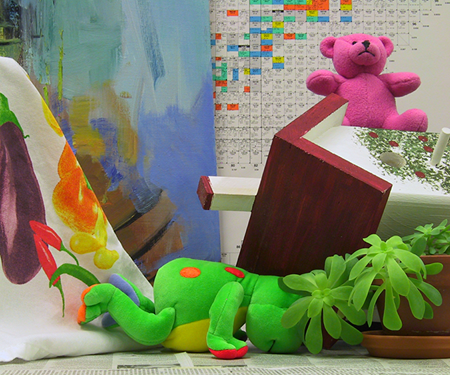
\includegraphics[width=1.2in,height=0.9in]{im2T.png}}
\subfigure[SAD diaparity]{\label{fig:subfig:b}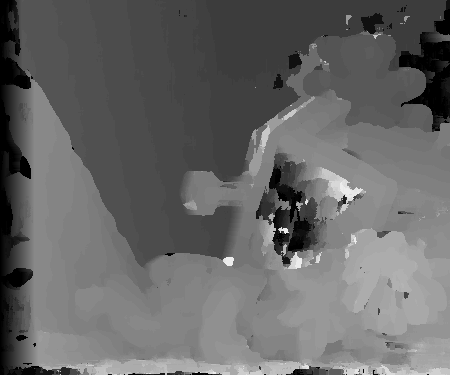
\includegraphics[width=1.2in,height=0.9in]{SADLeftT.png}}
\subfigure[SSD disparity]{\label{fig:subfig:b}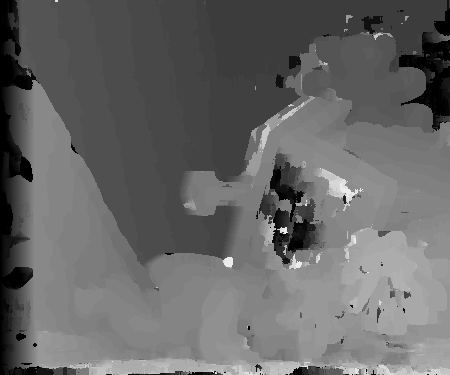
\includegraphics[width=1.2in,height=0.9in]{SSDLeftT.png}}
\subfigure[NCC disparity]{\label{fig:subfig:a}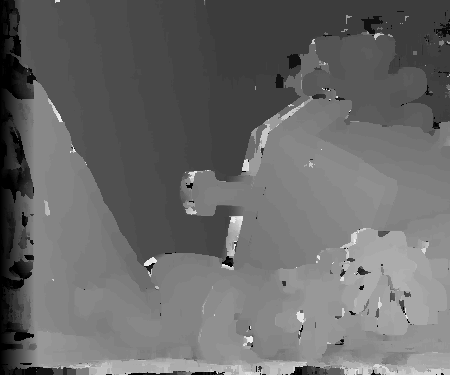
\includegraphics[width=1.2in,height=0.9in]{NCCLeftT.png}}
\subfigure[ASW diaparity]{\label{fig:subfig:b}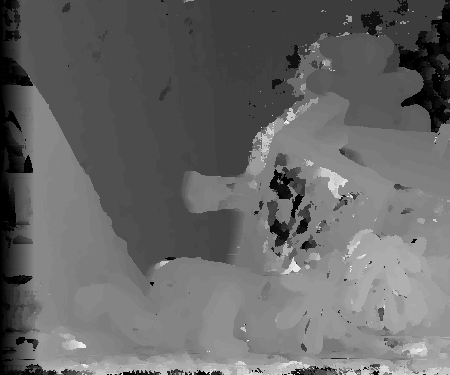
\includegraphics[width=1.2in,height=0.9in]{ASWLeftT.png}}
\subfigure[Standard disparity]{\label{fig:subfig:b}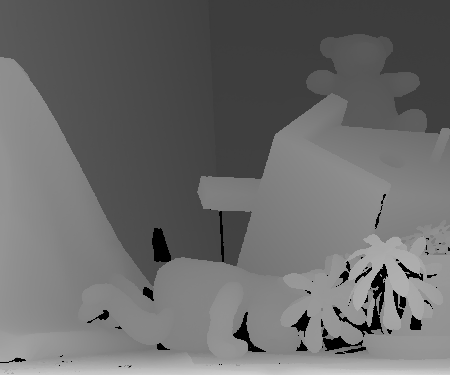
\includegraphics[width=1.2in,height=0.9in]{disp2T.png}}
\caption{Result of Teddy test pair}
\end{figure}
\end{frame}


\begin{frame}
\frametitle{4.1.1 Disparity maps of SAD, SSD, NCC and ASW}
Take Cones test pair for example, matching window $11\times11$

\begin{figure}
\centering
\subfigure[Left image]{\label{fig:subfig:a}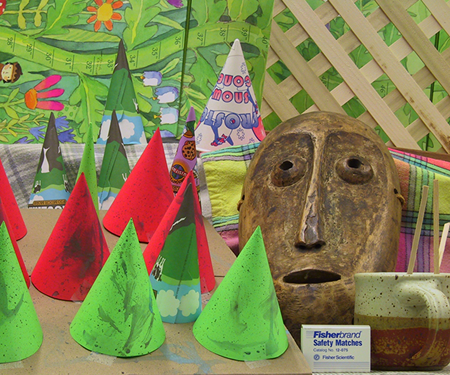
\includegraphics[width=1.2in,height=0.9in]{im2C.png}}
\subfigure[SAD diaparity]{\label{fig:subfig:b}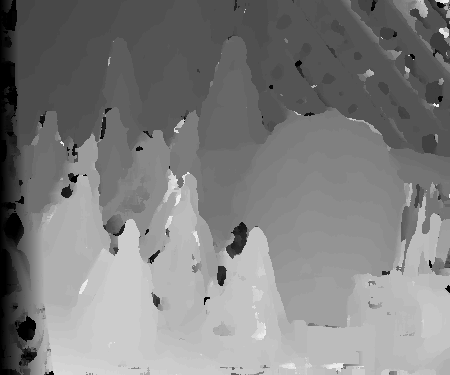
\includegraphics[width=1.2in,height=0.9in]{SADLeftC.png}}
\subfigure[SSD disparity]{\label{fig:subfig:b}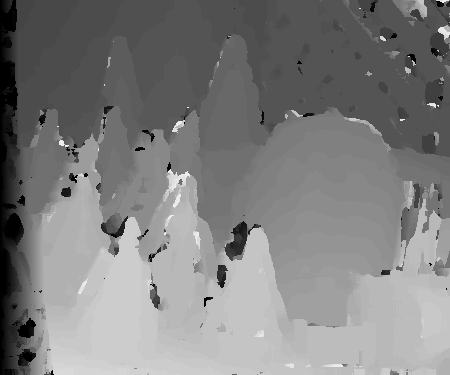
\includegraphics[width=1.2in,height=0.9in]{SSDLeftC.png}}
\subfigure[NCC disparity]{\label{fig:subfig:a}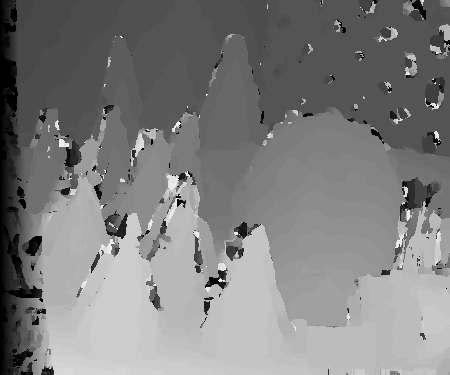
\includegraphics[width=1.2in,height=0.9in]{NCCLeftC.png}}
\subfigure[ASW diaparity]{\label{fig:subfig:b}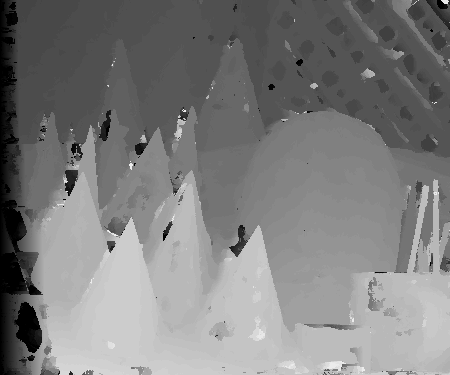
\includegraphics[width=1.2in,height=0.9in]{ASWLeftC.png}}
\subfigure[Standard disparity]{\label{fig:subfig:b}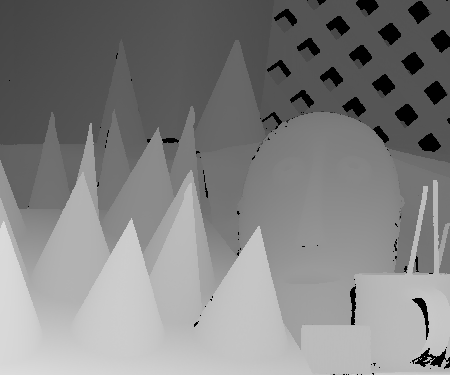
\includegraphics[width=1.2in,height=0.9in]{disp2C.png}}
\caption{Result of Cones test pair}
\end{figure}
\end{frame}


\begin{frame}
\frametitle{4.1.2 Contrast between four algorithms}
\raggedright Here are the false matching rate contrast of disparity maps generated by four algorithms

\begin{table}
\caption{False matching rate contrast (unit : percent)}
\begin{figure}[!htp]
\centering 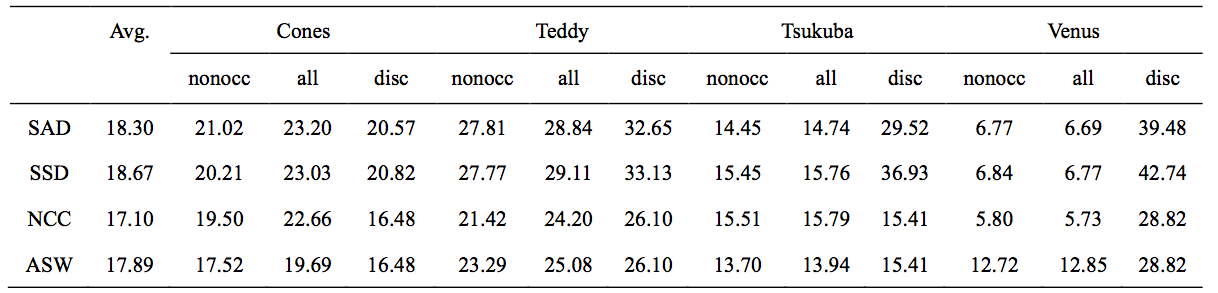
\includegraphics[width=4.5in]{ta1.png}
\end{figure}
\end{table}
where nonocc stands for non-occluded region, all stands for all region and disc stands for discontinuity region.

\end{frame}

\begin{frame}
\frametitle{4.1.2 Contrast between four algorithms}
\raggedright Here are the running time contrast of disparity maps generated by four algorithms

\begin{table}
\caption{Running time contrast (unit : second)}
\begin{figure}[!htp]
\centering 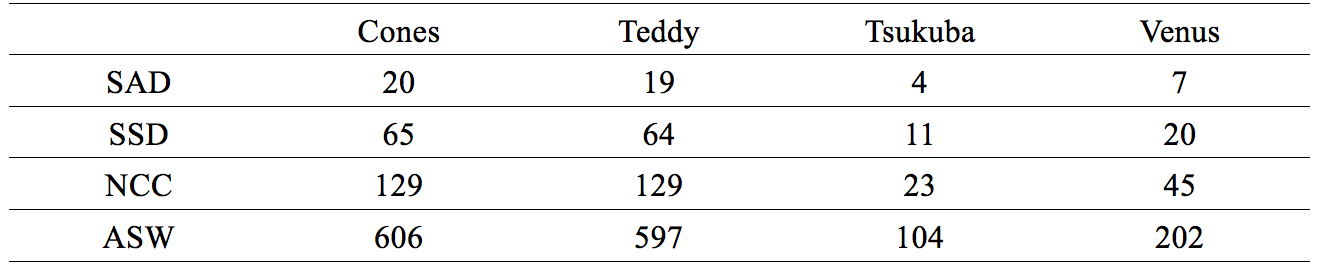
\includegraphics[width=4.5in]{s1.png}
\end{figure}
\end{table}

We can easily find that the running time of ASW $>$ NCC $>$ SSD $>$ $SAD$.
\end{frame}


\subsection{Design of optimization}
\begin{frame}
\frametitle{4.2 Design of optimization}

\begin{figure}[!htp]
\centering 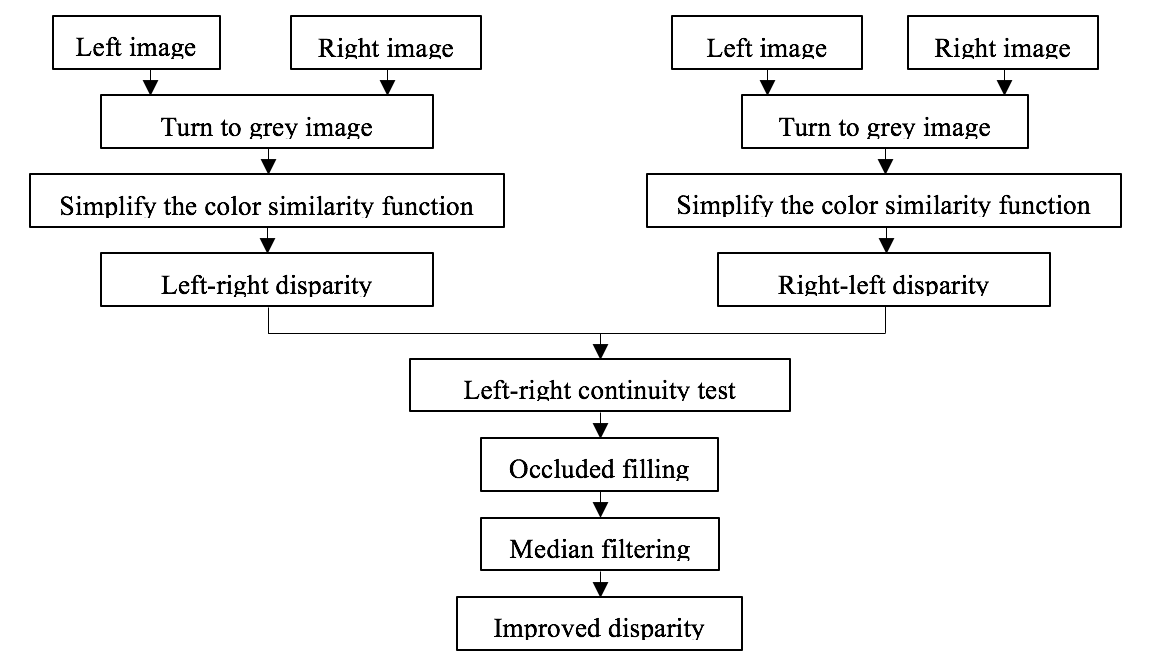
\includegraphics[width=5in, height=2.5in]{l1.png}
\caption{Design of Optimization}
\end{figure}
\end{frame}

\subsection{Experimental analysis of optimized algorithm}
\begin{frame}
\frametitle{4.3.1 Disparity maps of optimized algorithm}
Take teddy test pair for example, matching window $11\times11$

\begin{figure}
\centering
\subfigure[Left-right disparity]{\label{fig:subfig:b}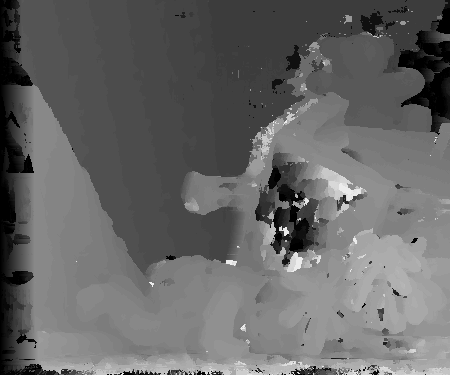
\includegraphics[width=1.3in,height=0.9in]{ASWLeft_teddy.png}}
\subfigure[Right-left disparity]{\label{fig:subfig:b}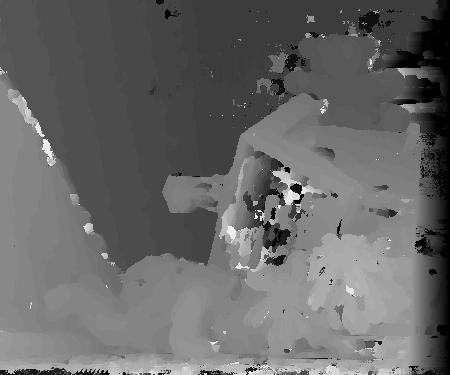
\includegraphics[width=1.3in,height=0.9in]{ASWRight_teddy.png}}
\subfigure[Occluded Region]{\label{fig:subfig:a}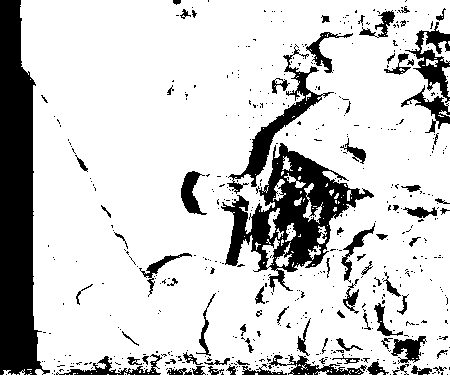
\includegraphics[width=1.3in,height=0.9in]{OccludedRegion.png}}
\subfigure[Occluded Filling]{\label{fig:subfig:b}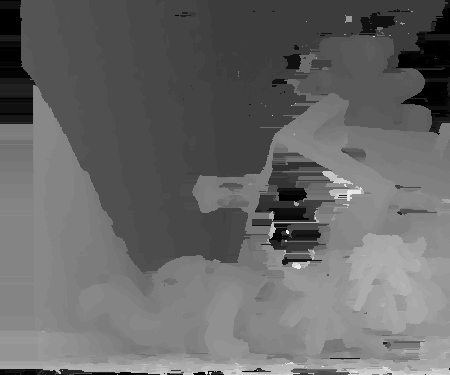
\includegraphics[width=1.3in,height=0.9in]{OccludedFilling.png}}
\subfigure[Median Filtering]{\label{fig:subfig:b}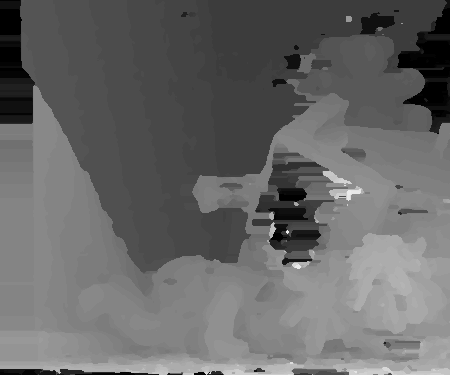
\includegraphics[width=1.3in,height=0.9in]{MedianFiltering.png}}
\subfigure[Standard disparity]{\label{fig:subfig:a}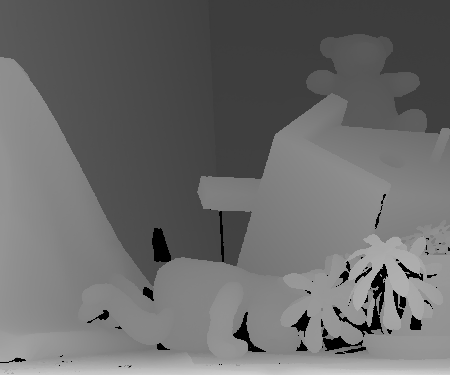
\includegraphics[width=1.3in,height=0.9in]{disp2T.png}}
\caption{Result of Teddy test pair}
\end{figure}
\end{frame}

\begin{frame}
\frametitle{4.3.2 Contrast of optimized algorithm and ASW algorithm}
Here are the contrast of optimized algorithm and ASW algorithm for test pair Teddy, Tsukuba and Venus.
\begin{figure}
\centering
\subfigure[ASW Teddy]{\label{fig:subfig:b}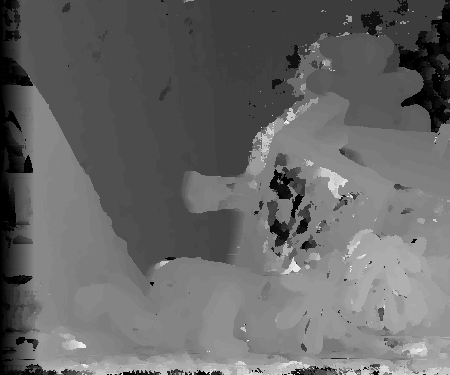
\includegraphics[width=1.3in,height=0.9in]{ASWLeftT.png}}
\subfigure[ASW Tsukuba]{\label{fig:subfig:b}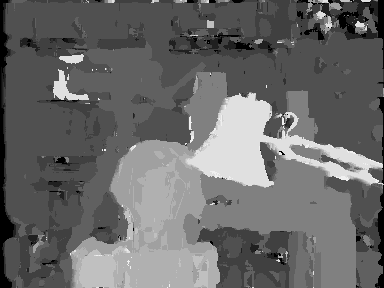
\includegraphics[width=1.3in,height=0.9in]{ASWLeftTsu.png}}
\subfigure[ASW Venus]{\label{fig:subfig:a}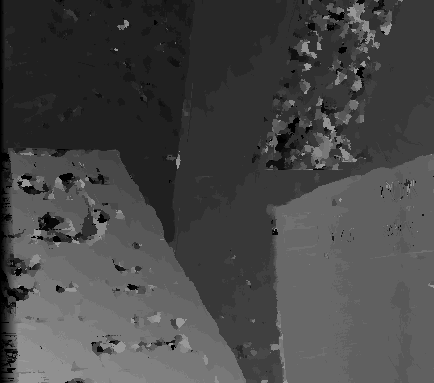
\includegraphics[width=1.3in,height=0.9in]{ASWLeftVen.png}}
\subfigure[Optim. Teddy]{\label{fig:subfig:b}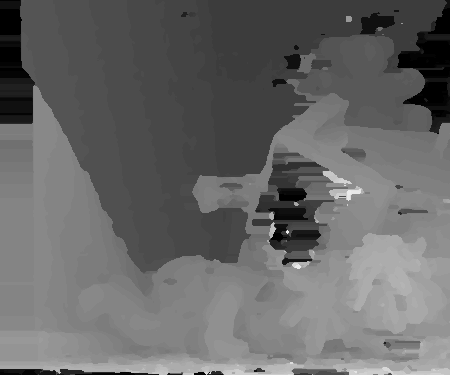
\includegraphics[width=1.3in,height=0.9in]{MedianFiltering.png}}
\subfigure[Optim. Tsukuba]{\label{fig:subfig:b}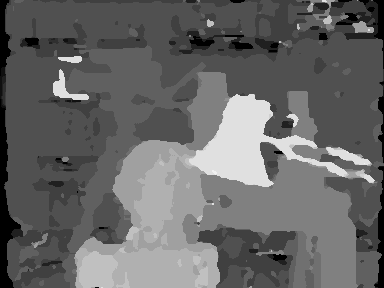
\includegraphics[width=1.3in,height=0.9in]{MedianFilteringTsu.png}}
\subfigure[Optim. Venus]{\label{fig:subfig:a}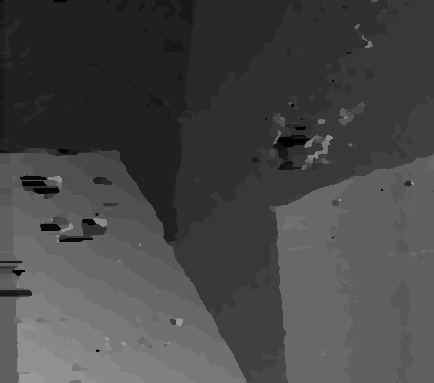
\includegraphics[width=1.3in,height=0.9in]{MedianFilteringVen.png}}
\caption{Contrast of two algorithms}
\end{figure}
\end{frame}


\begin{frame}
\frametitle{4.3.2 Contrast of optimized algorithm and ASW algorithm}
Here are the false matching rate contrast of optimized algorithm and ASW algorithm.

\begin{table}
\caption{False matching rate contrast (unit : percent) }
\begin{figure}
\centering
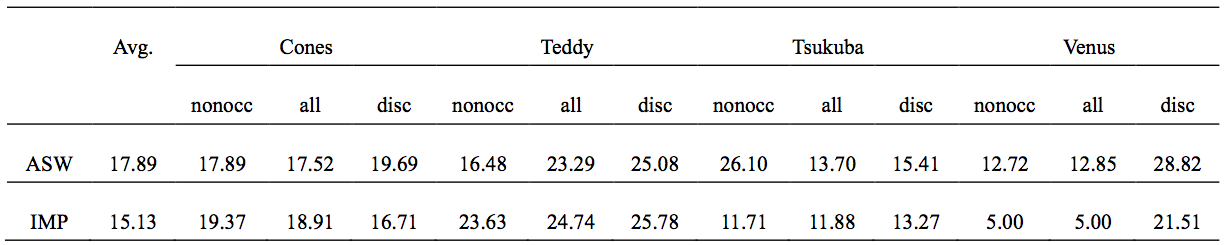
\includegraphics[width=4.5in]{p2.png}
\end{figure}
\end{table}

\raggedright Compared with the ASW algorithm, the false matching rate of optimized algorithm has reduced by 2.76 percent on average.
\end{frame}

\begin{frame}
\frametitle{4.3.2 Contrast of optimized algorithm and ASW algorithm}
Here are the running time contrast of optimized algorithm and ASW algorithm.
\begin{table}
\caption{Running time contrast (unit : second)}
\begin{figure}
\centering
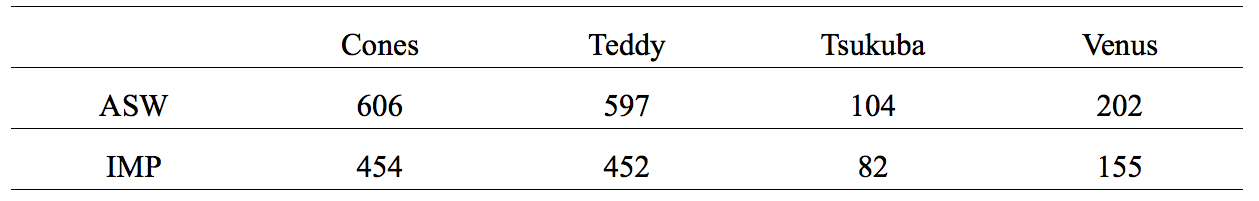
\includegraphics[width=4.5in]{p3.png}
\end{figure}

\end{table}

\raggedright Compared with the ASW algorithm, the running time of optimized algorithm has reduced by 20 percent on average.
\end{frame}

\subsection{Conclusion}
\begin{frame}
\frametitle{4.4 Conclusion}

\begin{enumerate}
\item By simplifying the color similarity function formula of the original ASW algorithm, the running time of program has reduced by 20 percent.

\item By performing the left and right consistency detection, occlusion filling and median filtering, the accuracy of disparity map has improved by 2.76 percent, 

\item The improved algorithm has good stereo matching accuracy on multi-texture region and multi-level region, and its matching accuracy of discontinuous region is better than that of original ASW algorithm.
\end{enumerate}

\end{frame}

\begin{frame}
\centering
\LARGE Thank you !
\end{frame}

\end{document}
